\begin{figure}[H]
    \centering
    \begin{minipage}[b]{0.4\textwidth}
        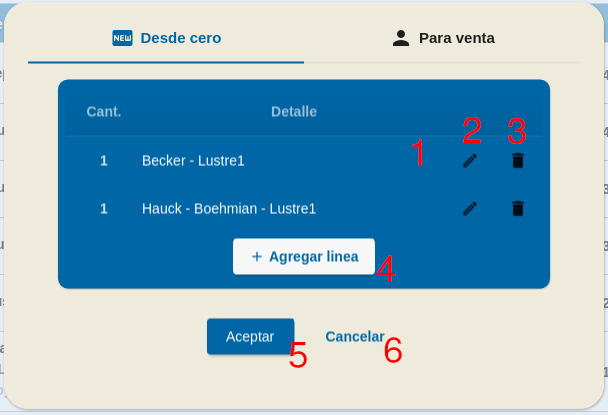
\includegraphics[width=\textwidth,height=\textheight,keepaspectratio]{Escenarios/AD-23-00-DesdeCero}
        \caption{AD-23-00 Desde cero}
        \label{fig:OrdenDesdeCero}
    \end{minipage}
    \hfill
    \begin{minipage}[b]{0.4\textwidth}
        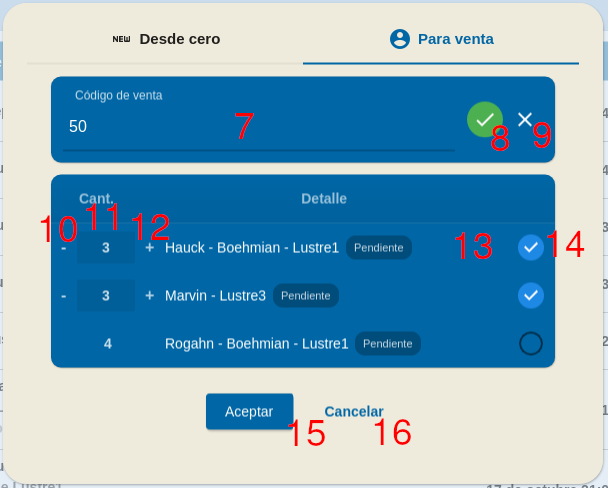
\includegraphics[width=\textwidth,height=\textheight,keepaspectratio]{Escenarios/AD-23-00-Venta}
        \caption{AD-23-00 Para venta}
        \label{fig:OrdenParaVenta}
    \end{minipage}
    \end{figure}

Este escenario permite a los usuarios crear/modificar una orden de producción. En caso de estar creando/modificando una orden de producción que no es para una venta se mostrará el contenido de la figura \ref{fig:OrdenDesdeCero} y en caso de estar creando/modificando una orden de producción que es para una venta se mostrará el contenido de la figura \ref{fig:OrdenParaVenta}. En la parte superior se muestran dos botónes para navegar entre estos dos contenidos 'Desde cero' o 'Para venta', los cuales no aparecerán si se está modificando una orden de producción. 

En caso de ser una orden de producción que no es para una venta. En \textbf{AD-23-01} se muestran las líneas de orden de producción que posee actualmente la orden de producción. En caso de no contar con ninguna linea se muestra un texto informando que debe ingresar al menos una linea. El botón \textbf{AD-23-02} permite modificar una linea de orden de producción, navegando al escenario \textbf{AD-24-00}. El botón \textbf{AD-23-03} permite borrar la linea de la orden de producción. El botón \textbf{AD-23-04} permite crear una nueva linea de orden de producción, navegando al escenario \textbf{AD-24-00}. El botón \textbf{AD-23-05} creará o modificará la orden de producción según corresponda y el botón \textbf{AD-23-06} cancelará la operación

En caso de ser una orden de producción para una venta, el campo \textbf{AD-23-07} permite ingresar el código de una venta existente, el botón \textbf{AD-23-08} permite traer las líneas de la venta según el código de venta ingresado en \textbf{AD-23-07} y el botón \textbf{AD-23-09} permite eliminar el texto ingresado en el campo \textbf{AD-23-07}. En caso de que el campo \textbf{AD-23-07} se encuentre vacío los botónes \textbf{AD-23-08} y \textbf{AD-23-09} se encontrarán inhabilitados. 
En \textbf{AD-23-13} se muestra las líneas de venta con su cantidad, mueble y estado actual. En el campo \textbf{AD-23-11} se puede modificar la cantidad a producir de un determinado mueble, pudiendo incrementar y decrementar dicha cantidad con los botónes \textbf{AD-23-12} y \textbf{AD-23-10} respectivamente. El botón \textbf{AD-23-14} permite indicar que se desea producir la cantidad especificada del mueble seleccionado. Si una linea no se encuentra seleccionada, la cantidad no se tiene en cuenta.
El botón \textbf{AD-23-15} creará o modificará la orden de producción para la venta especificada y el botón \textbf{AD-23-16} cancelará la operación.
\clearpage
